\documentclass[../main/main.tex]{subfiles}

\begin{document}

\section*{Introduction}

In this experiment we will look at the transient response of an RC-circuit and its properties as a frequency filter.
We will test the characteristics of the circuit using a square wave and a sinusiodal pulse.
Using the data obtained by the digital oscilloscope, we will determine the time constant \( \tau = RC \) experimentally, the scaling function \( g(f) \) and the phase shift \( \phi(f) \)

\section*{Theory}

\subsection*{Direct current}

The square wave behaves like direct current in the period of time, where the current is at a stable level.
This means that we can apply Kirchhoffs laws for direct current.

For the system in Fig.\ref{fig:setup}, Kirchhoffs law states the following

\begin{equation}
  \mathcal{E} = IR+\frac{1}{C} \int I(t) \dd t
\end{equation}

and we can differentiate to get the following

\begin{equation}
  0 = \dot{I} R + \frac{1}{C} I
\end{equation}

Solving this differential equation with the boundary condition that \( I(0) = \mathcal{E} / R \) gives us

\begin{equation}
  I(t) = \frac{\mathcal{E}}{R} e^{-\frac{1}{RC} t}
\end{equation}

Using \( U = RI \) we can find the voltage drop over the resistor

\begin{equation}
  U_R = \mathcal{E} e^{-\frac{1}{RC} t}
\end{equation}

If we want to find the voltage drop over the capacitor, we know that \( U_C = Q / C = \frac{1}{C} \int I(t) \dd t \).
Solving this with the boundary condition \( U_C(0) = 0 \) we get

\begin{equation}
  U_C = \mathcal{E} \left( 1 - e^{- \frac{1}{RC} t} \right)
\end{equation}

\subsection*{Alternating current}

For a RC-circuit as in Fig.\ref{fig:setup} the following apply according to Kirchhoffs laws

\begin{equation}
	\tilde{U}(t) = \tilde{I}(t)Z
\end{equation}

where \( \tilde{U} \) is the complex voltage, \( \tilde{I} \) is the complex current and \( Z \) is the impedance. Then we have the complex current

\begin{equation}
	\tilde{I}(t) = \frac{\tilde{U}(t)}{Z} = \frac{\tilde{U}(t)}{ \abs{Z}} e^{-i \phi}
\end{equation}

with \( Z = R + i/ \omega C \) where \( R \) is the resistance, \(\omega \) is the angular frequency and \( C \) is the capacitance.
If we write \( Z \) in polar coordinates we get the form \( Z = \abs{Z} e^{i \phi} \) where \( \abs{Z} = \sqrt{R^2 + (1/\omega C)^2} \) and \( \phi = \arctan(1 / R \omega C ) \)

We want to find the voltage drop over the resistance

\begin{equation}
	\tilde{U}_R(t) = R \tilde{I}(t) = R \frac{\tilde{U}(t)}{ \abs{Z}} e^{-i \phi}
\end{equation}

We know that our alternating complex voltage is \( \tilde{U}(t) = V_0 e^{-i \omega t } \).
We now want to find the real voltage

\begin{equation}
	U_R(t) = \mathcal{R}[\tilde{U}_R(t)] = R \frac{1}{ \sqrt{R^2 + \left( \frac{1}{ \omega C } \right)^2 } } V_0 \cos ( \omega t + \phi)
\end{equation}

The factor \( g = R / \sqrt{R^2 + ( 1 / \omega C )^2} \) is a scaling factor between the input voltage and the voltage drop over the resistor.
We see that a small \( \omega \) will result in a small \( g \) meaning that the voltage drop over the resistor will be smaller than the input voltage, the voltage is strongly damped.
For large \( \omega \), \( g \) will approach 1, so almost no damping.

The phase shift is \( \phi = \arctan( \frac{1}{ \omega RC })\).

In this experiment we will work with a resistance \( R = 1000 \Omega \) and capacitance \( C = 47 \si{\nano\farad} \).
We can anticipate a behavior for \( g \) as a function of \( \omega \) as depicted in Fig.\ref{fig:g_af_omega}.

Furthermore we can anticipate a behaviour for \( \phi \) as depicted in Fig.\ref{fig:phi_af_omega}

\begin{figure}[!ht]
  \centering
    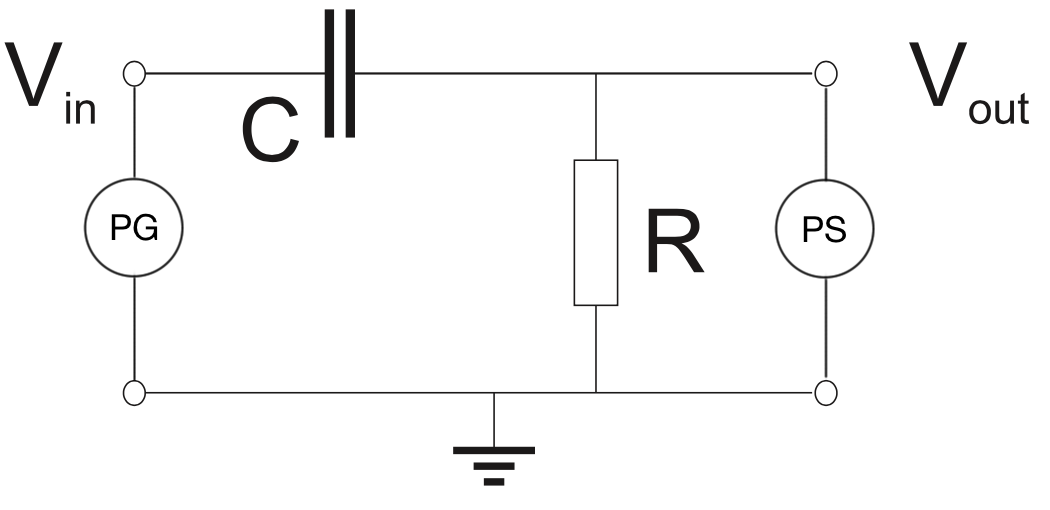
\includegraphics[width=0.7\textwidth]{../img/setup.png}
    \label{fig:setup}
    \caption{Setup for high pass filter}
\end{figure}

\begin{figure}[!ht]
  \caption{}
  \centering
  \begin{subfigure}[b]{0.4\textwidth}
      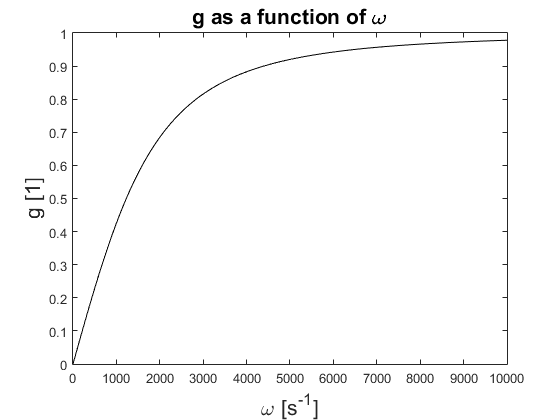
\includegraphics[width=\textwidth]{../img/g_af_omega.png}
      \caption{\( g \) as a function of \( \omega \)}
      \label{fig:phi_af_omega}
  \end{subfigure}
  ~ %add desired spacing between images, e. g. ~, \quad, \qquad, \hfill etc.
    %(or a blank line to force the subfigure onto a new line)
  \begin{subfigure}[b]{0.4\textwidth}
      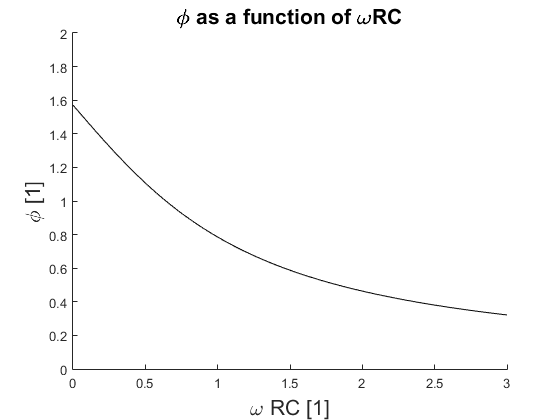
\includegraphics[width=\textwidth]{../img/phi_af_wRC.png}
      \caption{\( \phi \) as a function of \( \omega R C \)}
      \label{fig:g_af_omega}
  \end{subfigure}
  \caption{Scaling factor and \( \phi \) for the high pass filter}
\end{figure}

\section*{Setup}

The setup is as in Fig.\ref{fig:setup} with PG representing a pulse generator and PS representing a Picoscope which is a digital oscilloscope.
With the oscilloscope, we are measuring the voltage drop over the resistor.

We are using a resistor with resistance \( R = 10 \si{\kilo\ohm} \) and a capacitor with capacitance \( C = 47 \si{\nano\farad} \).

\section{Experiments}

For the following experiments we make use of a resistor and capacitor with the characteristics listed in Table.\ref{components}.

\begin{table}[]
\centering
\caption{Components used in the experiment}
\label{components}
\begin{tabular}{|l|l|l|}
\hline
          & Value                         & Uncertainty                  \\ \hline
Resistor  & \( 9.947 \si{\kilo\ohm} \)  & \( 0.001 \si{\kilo\ohm} \) \\ \hline
Capacitor & \( 47.2 \si{\nano\farad} \) & \( 0.1 \si{\nano\farad} \) \\ \hline
\end{tabular}
\end{table}

\subsection*{High pass and low pass filter, square wave}

We know that the capacitor will be charged with time, so we should be able to find a frequency of the square wave where the capacitor is almost fully charged and fully discharged within the time of the pulse width.
As the capacitor is charged, the voltage drop over the resistor will increase, and decrease as the capacitor is discharged.
When a useful frequency and pulse width is determined, we get a good representation of the curve of the voltage drop over the resistor or capacitor, depending on the current system configuration.
In Fig.\ref{fig:VinVCVR} we see the input voltage and the corresponding voltage drop over the capacitor and resistor.
\( V_C \) represents the voltage drop over the capacitor, and \( V_R \) the voltage drop over the resistor.

\begin{figure}[!ht]
  \caption{Setup for high pass filter}
  \centering
    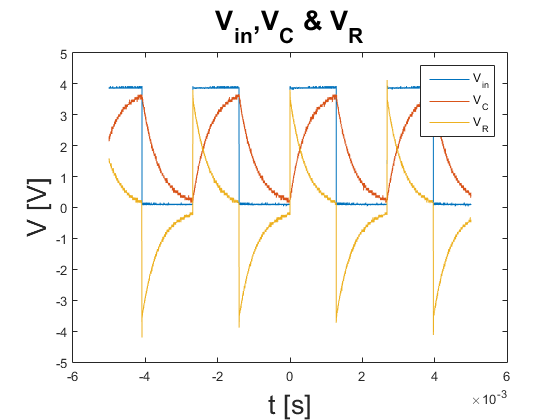
\includegraphics[width=0.7\textwidth]{../img/VinVCVR.png}
    \label{fig:VinVCVR}
\end{figure}

\subsection*{High pass filter, sine wave}

We replace the pulse generator with a function generator to produce an alternating current in the form of a sine wave.
The frequency is set as close as possible to \(  f = \omega_0 / 2 \pi = 340.4 \si{\hertz} \), where \( omega_0 \) is the angular frequency for the resonance, and the amplitude adjusted so that the input voltage measured on the Picoscope is \( 1 \si{\volt} \) peak-to-peak.

We then alternate the frequency from around \( 100 \si{\hertz} \) to \( 1000 \si{\hertz} \) and measure the output voltage and phase shift.
For each frequency we save the data in a txt file for later processing.
% See Fig.\ref{data} for measurements made directly in the software for the Picoscope.

% \begin{table}[!h]
% \centering
% \caption{Data from high pass filter, sine wave}
% \label{data}
% \begin{tabular}{|l|l|l|l|}
% \hline
% Frequency input [Hz]  & Peak to peak input [V]  & Peak to peak output [V]  & Phase shift [ms] \\
% \(\pm 5 \cdot 10^{-2}Hz\) & \(\pm 5\cdot 10^{-5}V\) & \(\pm 5 \cdot 10^{-5}V\) & \(\pm 5\cdot 10^{-4}ms\) \\ \hline
% 108.0 & 1.040 & 0.4365 & 8.055 \\ \hline
% 201.1 & 1.048 & 0.5952 & 4.226 \\ \hline
% 300.5 & 1.040 & 0.7698 & 2.888 \\ \hline
% 339.4 & 1.040 & 0.8095 & 2.565 \\ \hline
% 400.5 & 1.040 & 0.8571 & 2.212 \\ \hline
% 500.6 & 1.048 & 0.9571 & 1.806 \\ \hline
% 599.4 & 1.040 & 0.9474 & 1.543 \\ \hline
% 699.0 & 1.048 & 1.0050 & 1.332 \\ \hline
% 901.1 & 1.049 & 1.0350 & 1.050 \\ \hline
% 999.9 & 1.048 & 1.0550 & 0.958 \\ \hline
% \end{tabular}
% \end{table}
% %%

\subsection{Low pass filter, sine wave}

For the last part of the experiment, we switch the capacitor and resistor and create a low pass filter, see Fig.\ref{fig:setup2}.

\begin{figure}[!ht]
  \centering
    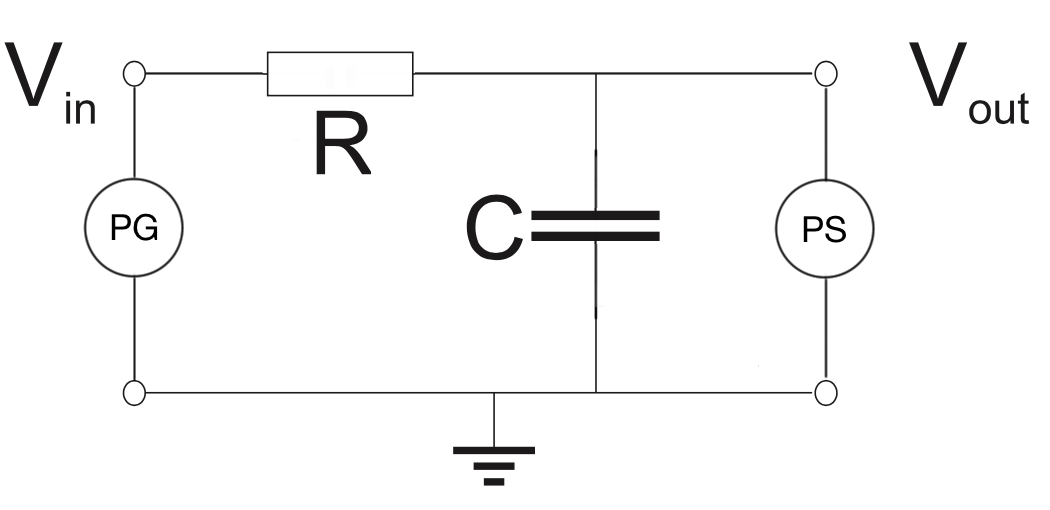
\includegraphics[width=0.7\textwidth]{../img/setup2.png}
    \label{fig:setup2}
    \caption{Setup for low pass filter}
\end{figure}

We perform the same measurements for the low pass filter, although the span for the frequencies is adjusted to get a useful representation of the behaviour of the circuit.

\section{Data processing}

\subsection*{Square wave}

To determine the time constant \( RC \) we fit the measured time dependent voltage drop over the resistor applying Eq.3.

\begin{table}[]
\centering
\caption{\( \tau = RC \) for the square wave system}
\label{data_square}
\begin{tabular}{|l|l|l|}
\hline
             & \( \tau = RC\) [s]       & Uncertainty [s]                         \\ \hline
Theoretical  & \( 4.70 \cdot 10^{-4} \) &                                         \\ \hline
Experimental & \( 4.3 \cdot 10^{-4} \)  & \( \pm 0.4 \cdot 10^{-4} \)             \\ \hline
Difference   & \( 0.4 \cdot 10^{-4} \)  &                                         \\ \hline
\end{tabular}
\end{table}

FIGUR MED FIT OG PARAMETRE

\subsection*{Alternating current}

We want to check the scaling factor \( g \) by plotting the output voltage as a function of \( \omega \).
Since the fit is an exponential function and the theoretically derived \( g \) is in another form, fitting an exponential curve to the measured data will make comparison difficult. So we will plot the measured output voltage againt the theoretical \( g \cdot V_{in} \), \( V_{in} \) begin the experimental value, and do a \( \chi^2 \) test to determine whether or not the measured values are within a acceptable range of the theory.
We arrive at the results in Table.CHI.I.ANDEN.FOR.G with a visual representation in Fig.\ref{fig:VinVudafphi}

\begin{figure}[!ht]
  \caption{ \( V_{out} \) as a function of \( \omega \) }
  \centering
    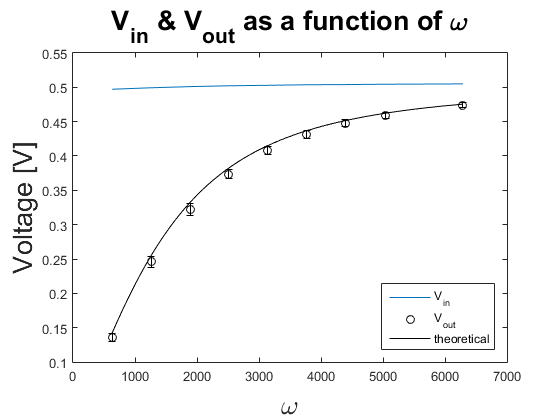
\includegraphics[width=0.7\textwidth]{../img/VinVudafphi.png}
    \label{fig:VinVudafphi}
\end{figure}

For the phase shift, we plot the phase as a function of \( \omega \).
As with \( g \) the fit will be on another form than the expression earlier determined for \( \phi \), so we will evaluate the measured results by plotting them with the theoretical values.
The results are presented in Table.CHI.I.ANDEN.FOR and in Fig.PLOT.AF.PHI.MOD.THEO

\section{Uncertainties}

The measurements have very limited uncertainties since the digital oscilloscope used is very precise.
In our calculations we have estimated the wires and contacts to be without any resistance which is not entirely correct.
As some plots obviously points out, many measurements are just below the theoretical value.
We estimate that we could probably hit the theoretical values even better, if we introduces an extra resistance representing the resistance in the wires, switches and so on.
Furthermore, the Picoscope is connected in parallel and has an internal resistance.
Although this resistance is far greater than for the rest of the circuit, some current will still run through it.
In our calculations all current runs through the resistor and capacitor.

\section{Conclusion}

The measurements are close to the theoretical values but not within range of the error.
Since the measurements are all shifted in the same direction a systematical error seems to be present.
NOT FINISHED

\section{References}

Taylor, J.R. (1997) An introduction to error analysis: The study of uncertainties in physical measurements. 2nd edn. United States: University Science Books,U.S.

\end{document}
